\documentclass[12pt]{beamer}
\usepackage[utf8]{inputenc}
\usepackage[spanish]{babel}
%\usepackage[dvips]{epsfig}
\usepackage{graphics}
\usepackage{url}
\usepackage{ulem}
\usepackage{beamerthemesplit}
\usepackage{color}
\usepackage{hyperref}
\usepackage{wrapfig}
\usetheme{CambridgeUS}
\setbeamercovered{transparent}

\title{User identification with username and password in structured P2P networks}
\subtitle{}
\author[R. Fernández]{Rodrigo Fernández \\ \small{\texttt{rfernand@inf.utfsm.cl}}}
\institute[]{Universidad Técnica Federico Santa María}
\titlegraphic{\includegraphics[height=1cm]{img/logo}}
\date{\today}


%- Problema
%- Porque el problema es importante
%  - Redes p2p solo identifican nodos-ip
%  - Explicar redes estructuradas para ello
%  - Necesario si es que uno quiere construir aplicaciones que requieran permisos a nivel de usuario
% \frametitle{Goals} ?
%- soluciones actuales
%  - PKI
%  - problemas de las mismas: alta probabilidad de falla. Riesgos ante
%    recuperacion de contraseñas
%- solucion
%  - building blocks
%   - acuerdo bizantino
%   - sistemas de reputacion: sistema que asigna un valor de reputacion a cada
%     nodo segun recomendaciones emitidas despues de cada transaccion.
%   - anillos de confianza: se requiere tambien un sistema que permita armar
%     sub-redes (anillos) con los nodos que posean una reputacion > delta, de tal
%     forma de generar una anillo de confianza. La solucion propuesta trabajara sobre
%     este anillo de confianza. Ej: CORPS
%  - protocolos
%  - justificacion del uso de los sistemas de confianza (comparacion del sistema
%    que no use esto)
%- conclusion: se comprueba la hipotesis gracias a los datos obtenidos
%  (grafico/tabla)
%- trabajo futuro
% - sistemas de recuperacion de contrasenas
% - ..



\begin{document}
\bibliographystyle{plain}
  \frame{\titlepage}
  \frame{\tableofcontents}
  \section{The problem and objectives of the research}
  \begin{frame}
\frametitle{P2P Networks}
\framesubtitle{Characteristics}
\begin{table}
\begin{tabular}{p{7cm}p{3cm}}
\begin{itemize}
  \item Scalable
  \item Decentralized
  \item Self-maintained
  \item Robust
\end{itemize}
&
\vspace{1.5cm}
\includegraphics[width=4cm]{img/p2p-unstructured}\\
\end{tabular}
\end{table}
\end{frame}

\begin{frame}
\frametitle{P2P Networks}
\framesubtitle{Overlay structure}
\begin{table}
\begin{tabular}{p{7cm}p{3cm}}
\begin{itemize}
    \item Structured networks (CAN, CHORD)
    \item Unstructured networks (Gnutella, Bittorrent)

\end{itemize}
&
\vspace{1.5cm}
\includegraphics[width=4cm]{img/p2p-structured}\\
\end{tabular}
\end{table}
\end{frame}

\begin{frame}
\frametitle{P2P Networks}
\framesubtitle{The problem}
\begin{table}
\begin{tabular}{p{7cm}p{3cm}}
\begin{itemize}
  \item P2P Networks only identify the nodes by their IP address 
\end{itemize}
&
\vspace{1.5cm}
\includegraphics[width=4cm]{img/p2p-structured}\\
\end{tabular}
\end{table}
\end{frame}

%- Problema
\begin{frame}
\frametitle{The problem (2)}
%\framesubtitle{Characteristics}
\begin{table}
\begin{tabular}{p{7cm}p{3cm}}
\begin{itemize}
  \item Existing systems manage \textbf{user-level permission} by issuing \textbf{pre-shared keys}.
  \item This does \textbf{not provide the flexibility} that a username-password based identification provides.
\end{itemize}
&
\vspace{1.5cm}
%\includegraphics[width=4cm]{img/p2p-unstructured}\\
\begin{itemize}
  \item Access from \textbf{Multiple devices}?
  \item \textbf{Key handling}
\end{itemize}
\end{tabular}
\end{table}
\end{frame}


\begin{frame}
\frametitle{The problem (3)}
%\framesubtitle{Characteristics}
\begin{table}
\begin{tabular}{p{7cm}p{3cm}}
\begin{itemize}
  \item The use of a \textbf{username and a password} means that the \textbf{user keys} needs to be \textbf{secured inside} the identification system
  \item While a \textbf{solution} has been proposed before, it does \textbf{not} take in
consideration the presence of \textbf{malicious nodes}
\end{itemize}
&
\vspace{1.5cm}
%\includegraphics[width=4cm]{img/p2p-unstructured}\\
\end{tabular}
\end{table}
\end{frame}

\begin{frame}
%- Porque el problema es importante
\frametitle{Why this is important?}
%  - Redes p2p solo identifican nodos-ip
%  - Explicar redes estructuradas para ello
%  - Necesario si es que uno quiere construir aplicaciones que requieran
%    permisos a nivel de usuario
%\framesubtitle{Characteristics}
\begin{table}
\begin{tabular}{p{7cm}p{3cm}}
\begin{itemize}
  \item \textbf{Applications that need user-level permissions need a way to identify users}
\end{itemize}
&
\vspace{1.5cm}
\includegraphics[width=4cm]{img/users}\\
\end{tabular}
\end{table}
\end{frame}



\begin{frame}
\frametitle{Goals}
%\framesubtitle{Characteristics}
\begin{table}
\begin{tabular}{p{7cm}p{3cm}}
\begin{itemize}
  \item Analize the security risks in using username/password identification in P2P networks. 
  \item Check the different security schemes that can be used in a P2P network with malicious nodes.
  \item Propose a P2P username/password identification system.
\end{itemize}
&
\vspace{1.5cm}
%\includegraphics[width=4cm]{img/p2p-unstructured}\\
\end{tabular}
\end{table}
\end{frame}

  \label{sec:goals}
  \section{Theoretical framework}
  \begin{frame}
\frametitle{Redes P2P}
\begin{table}
\begin{tabular}{p{7cm}p{3cm}}
\begin{itemize}
    \item ...
\end{itemize}
&
\vspace{1.5cm}
\includegraphics[width=4cm]{img/example}\\
\end{tabular}
\end{table}
\end{frame}

  \label{sec:soa}
  \begin{frame}
\frametitle{Methodology}
\framesubtitle{}
\begin{table}
\begin{tabular}{p{7cm}p{3cm}}
\begin{itemize}
  \item The goal of our approach was to drastically reduce the probability of a
malicious node impersonating another user who is using the identification
system. This was done using of a reputation system and trusted node management
to mitigate the effectivity of malicious nodes on identity usurpation attacks.

\end{itemize}
&
\vspace{1.5cm}
\includegraphics[width=4cm]{img/example}\\
\end{tabular}
\end{table}
\end{frame}

  \section{Findings}
  \label{sec:findings}
  \subsection{Building blocks}
\begin{frame}
\frametitle{Findings}
\framesubtitle{Building blocks}
\begin{table}
\begin{tabular}{p{7cm}p{3cm}}
\begin{itemize}
  \item DHT based (Pastry)
  \item Each node has its own pair of Pub/Priv keys
  \item Simple storage system
  \item Reputation system (WTR + CORPS)
  \item Challenges and computational puzzles
    % CORPS builds a double ring inside the DHT to find the most trustworthy node to a key K
  \item System protocols
\end{itemize}
&
\vspace{1.5cm}
\includegraphics[width=4cm]{img/example}\\
\end{tabular}
\end{table}
\end{frame}

\subsection{System protocols}
\begin{frame}
\frametitle{System protocols}
%\framesubtitle{Building blocks}
\begin{table}
\begin{tabular}{p{7cm}p{3cm}}
\begin{itemize}
  \item Securing the nodes of a leafset
  \item Account registration
  \item User sign in
  \item Logout
  \item Password Change
  \item User private key recovery
\end{itemize}
&
\vspace{1.5cm}
\includegraphics[width=4cm]{img/example}\\
\end{tabular}
\end{table}
\end{frame}

\subsection{Securing the nodes of a leafset}
\begin{frame}
\frametitle{System protocols}
\framesubtitle{Securing the nodes of a leafset}
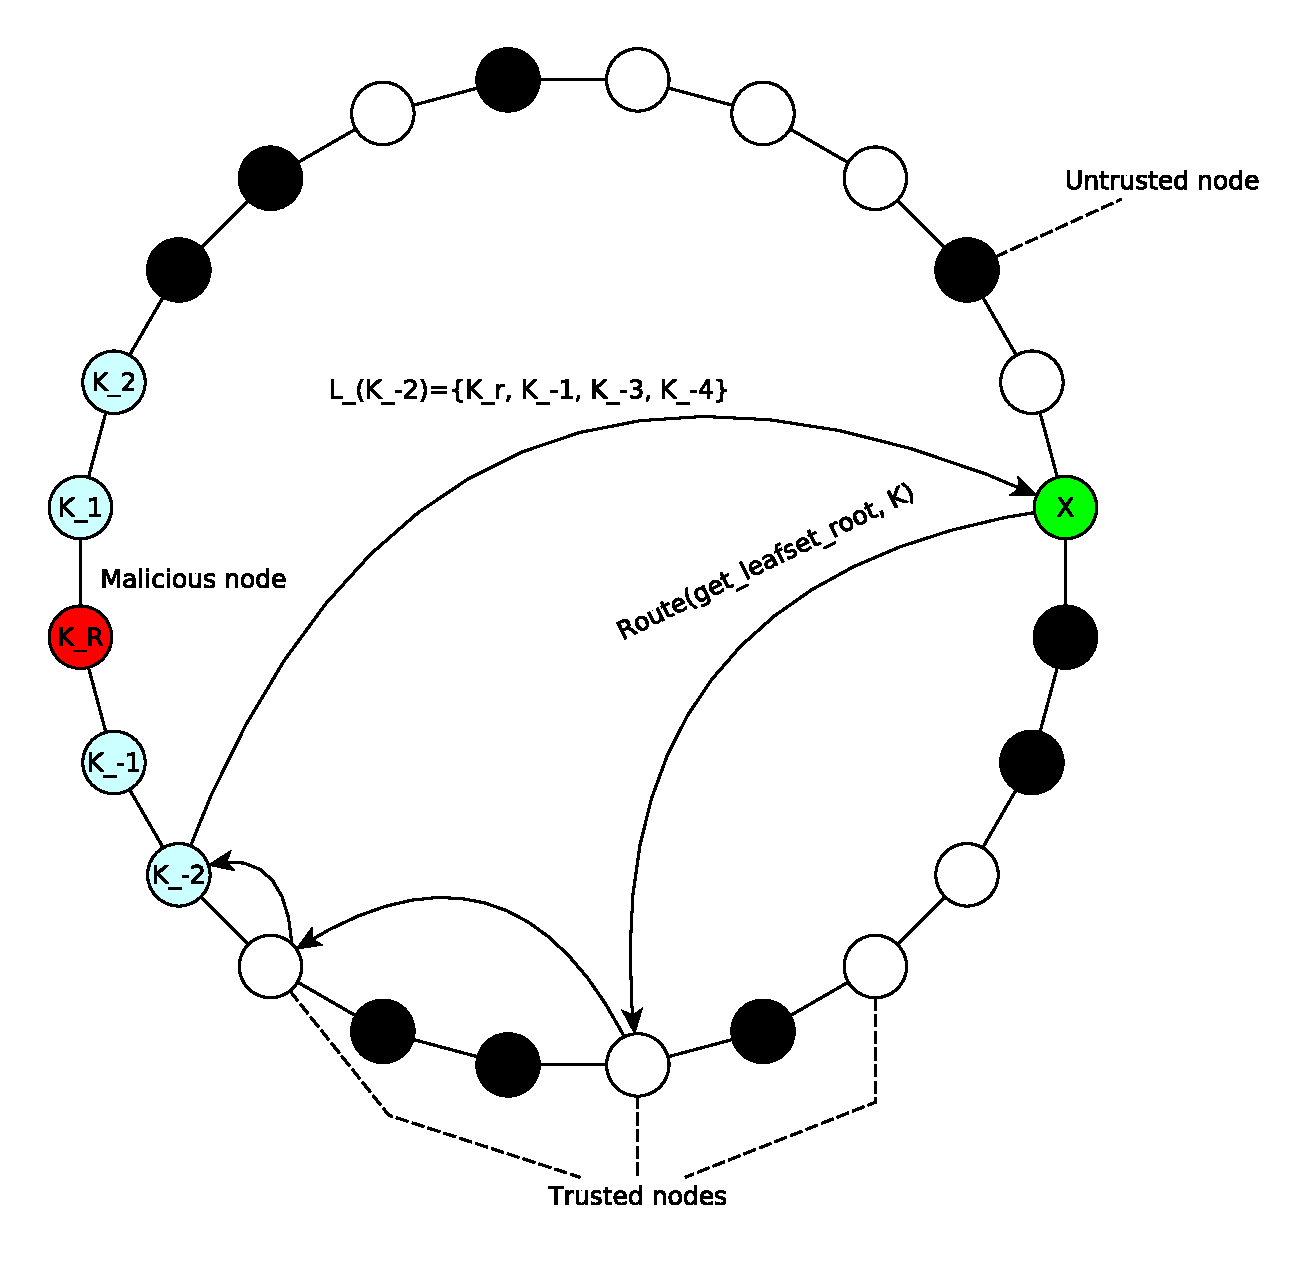
\includegraphics[height=0.7\textheight]{../../img/secure_routing}\\
%\begin{table}
%\begin{tabular}{p{7cm}p{3cm}}
%&
%\vspace{1.5cm}
%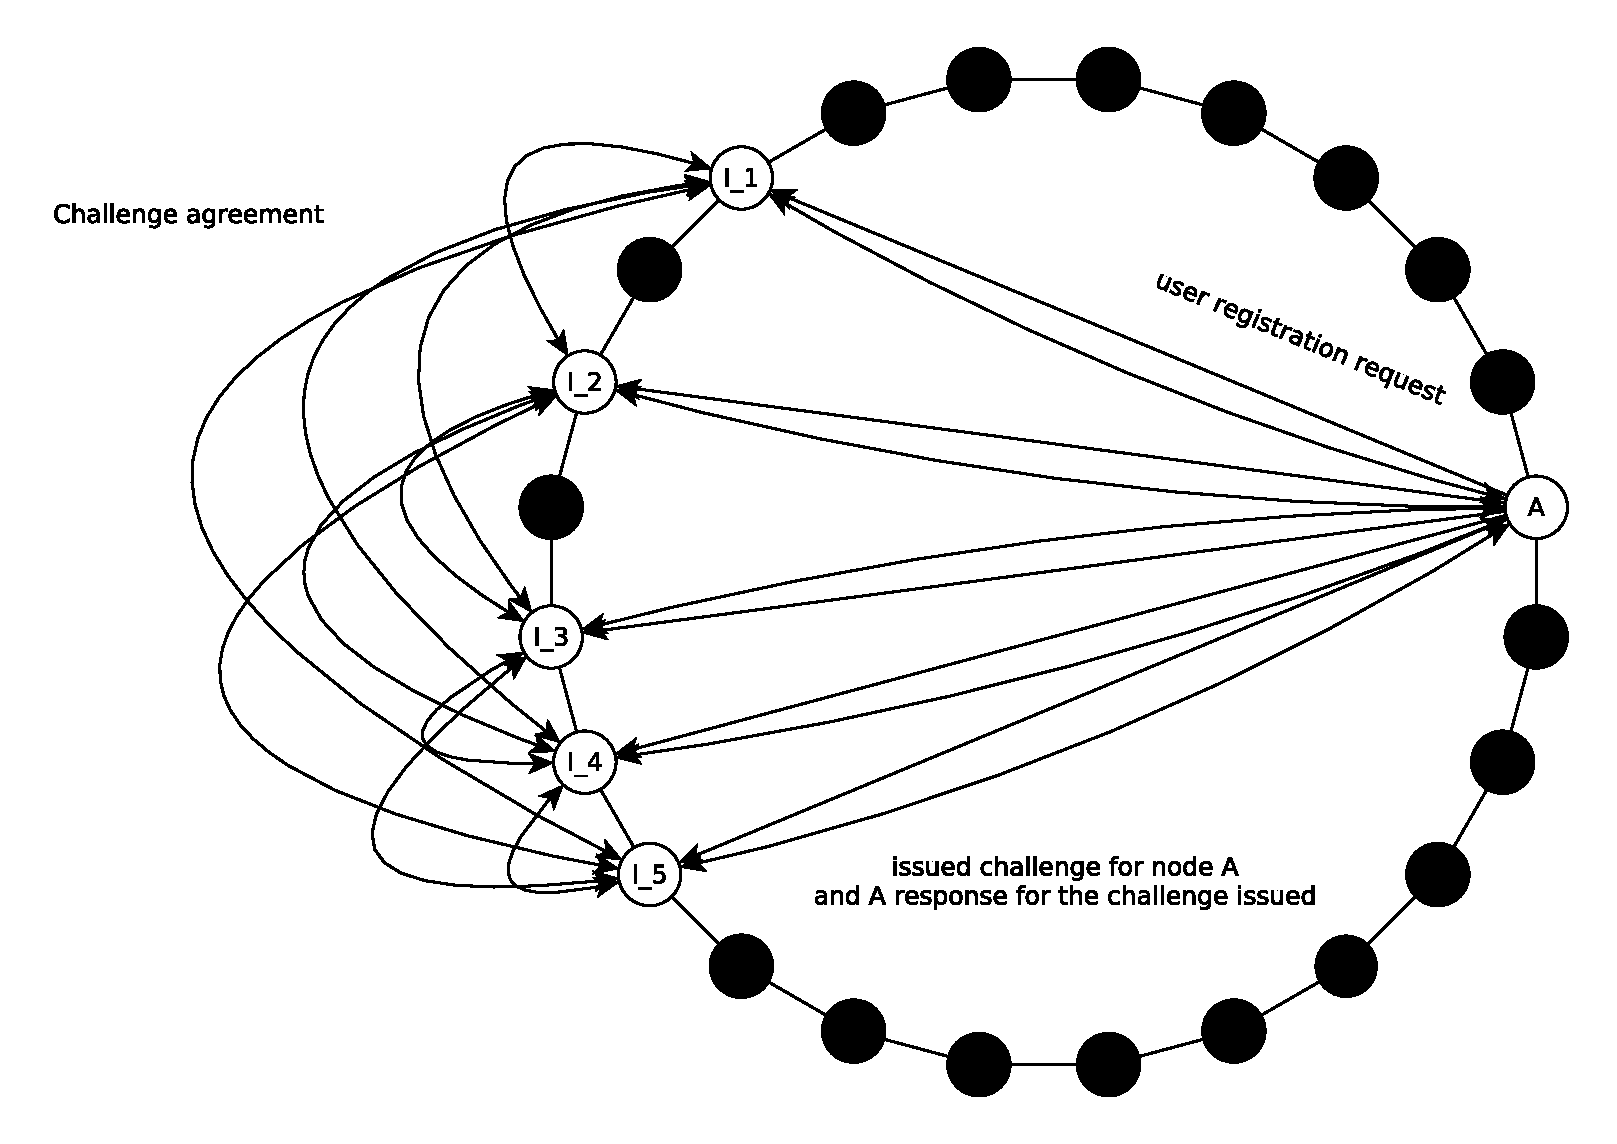
\includegraphics[width=4cm]{../../img/sign_up}\\
%\end{tabular}
%\end{table}
\end{frame}

\subsection{Account registration}
\begin{frame}
\frametitle{System protocols}
\framesubtitle{Account Registration}
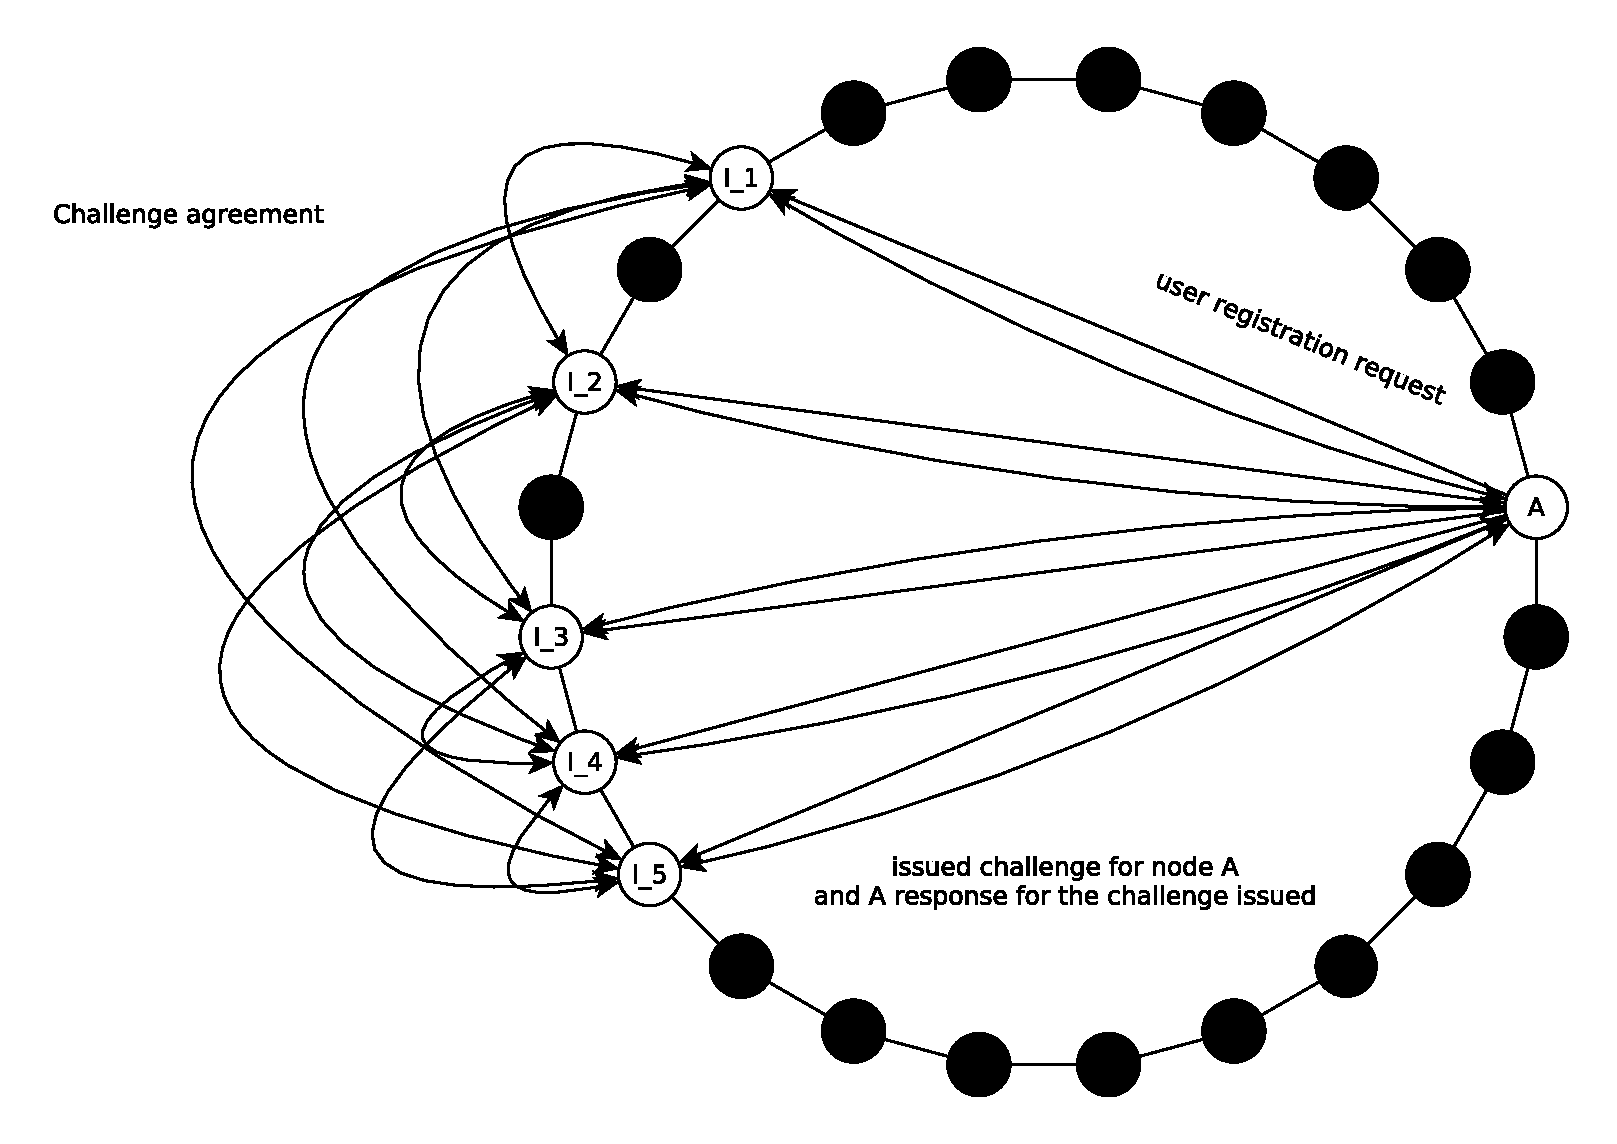
\includegraphics[height=0.7\textheight]{../../img/sign_up}\\
%\begin{table}
%\begin{tabular}{p{7cm}p{3cm}}
%&
%\vspace{1.5cm}
%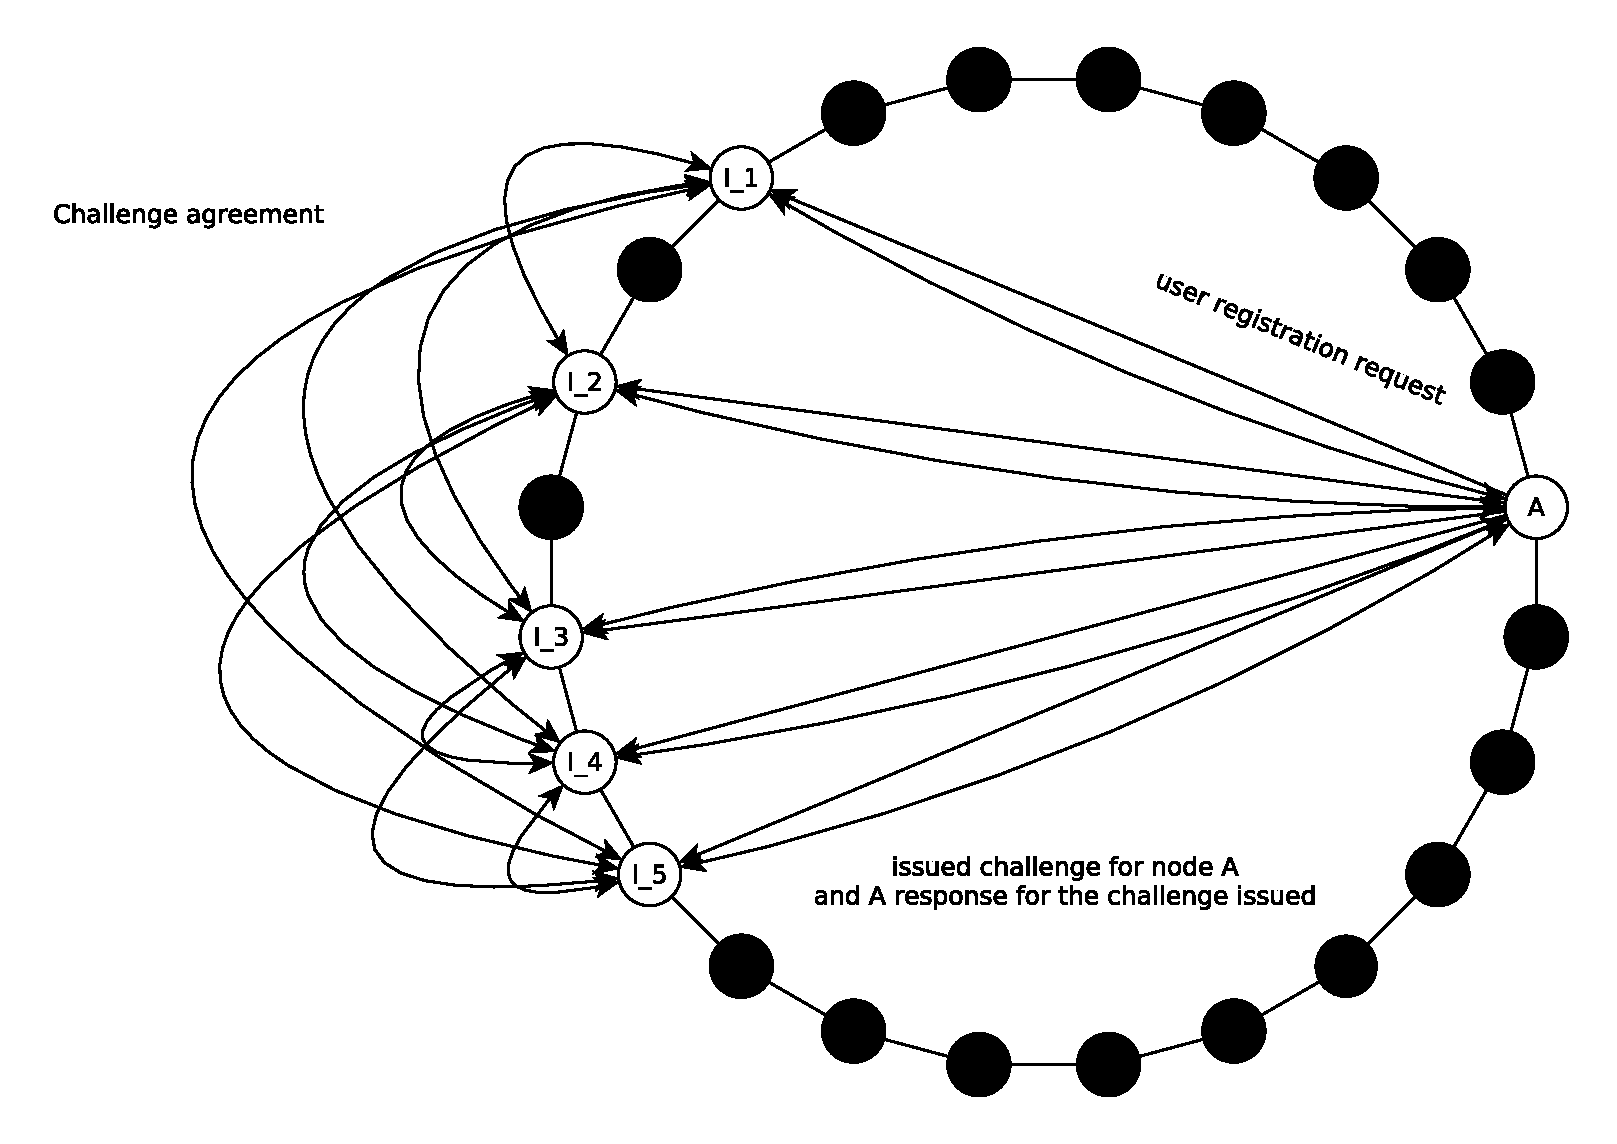
\includegraphics[width=4cm]{../../img/sign_up}\\
%\end{tabular}
%\end{table}
\end{frame}

\subsection{User sign in}
\begin{frame}
\frametitle{System protocols}
\framesubtitle{User sign in (Start)}
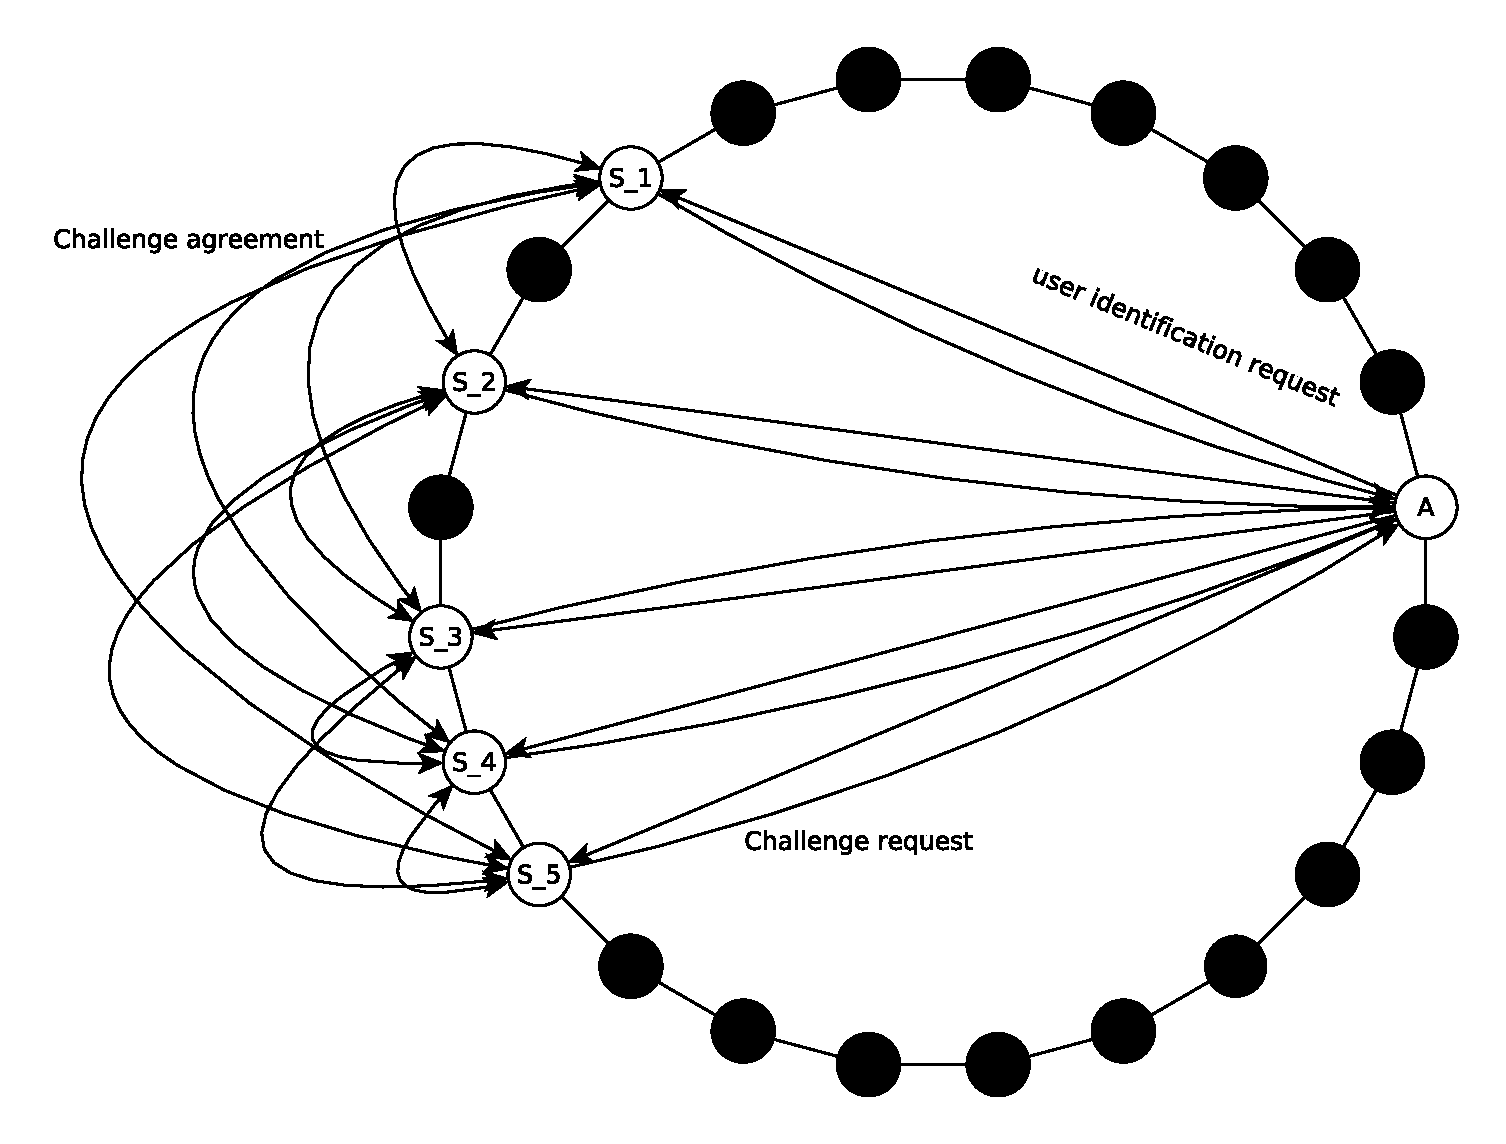
\includegraphics[height=0.7\textheight]{../../img/sign_in}\\
%\begin{table}
%\begin{tabular}{p{7cm}p{3cm}}
%&
%\vspace{1.5cm}
%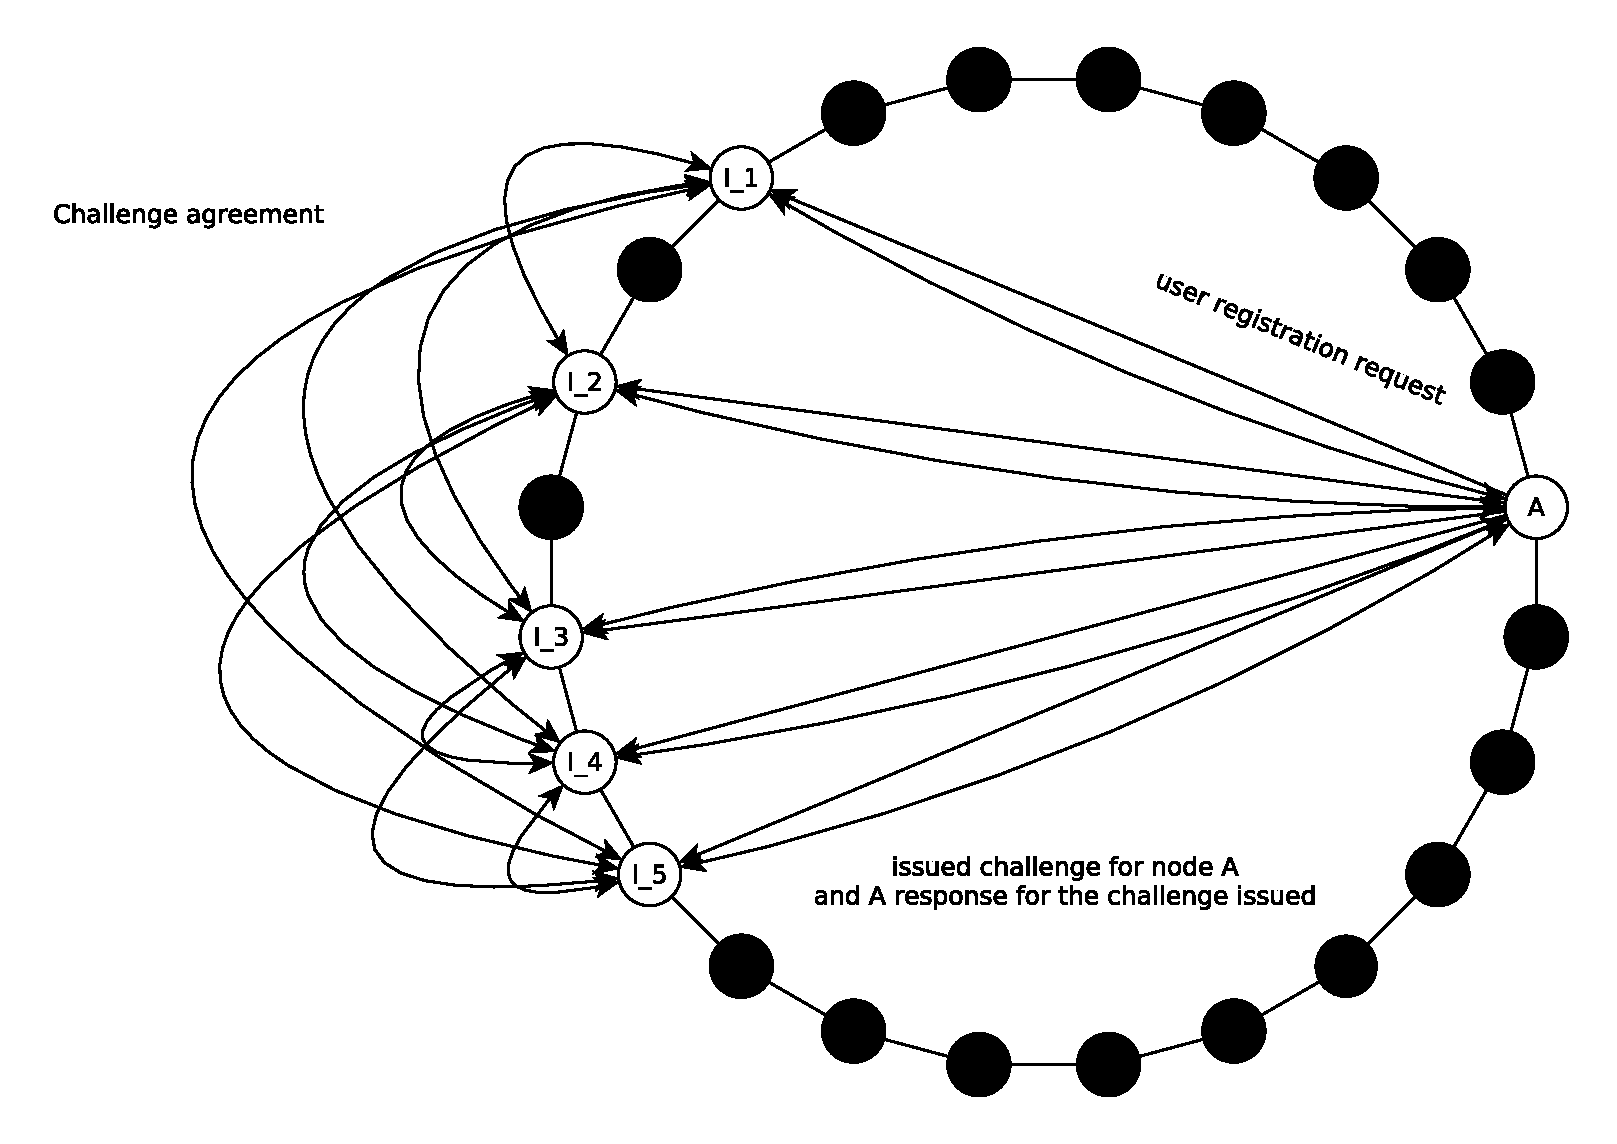
\includegraphics[width=4cm]{../../img/sign_up}\\
%\end{tabular}
%\end{table}
\end{frame}

\begin{frame}
\frametitle{System protocols}
\framesubtitle{User sign in (Retrieve of public key)}
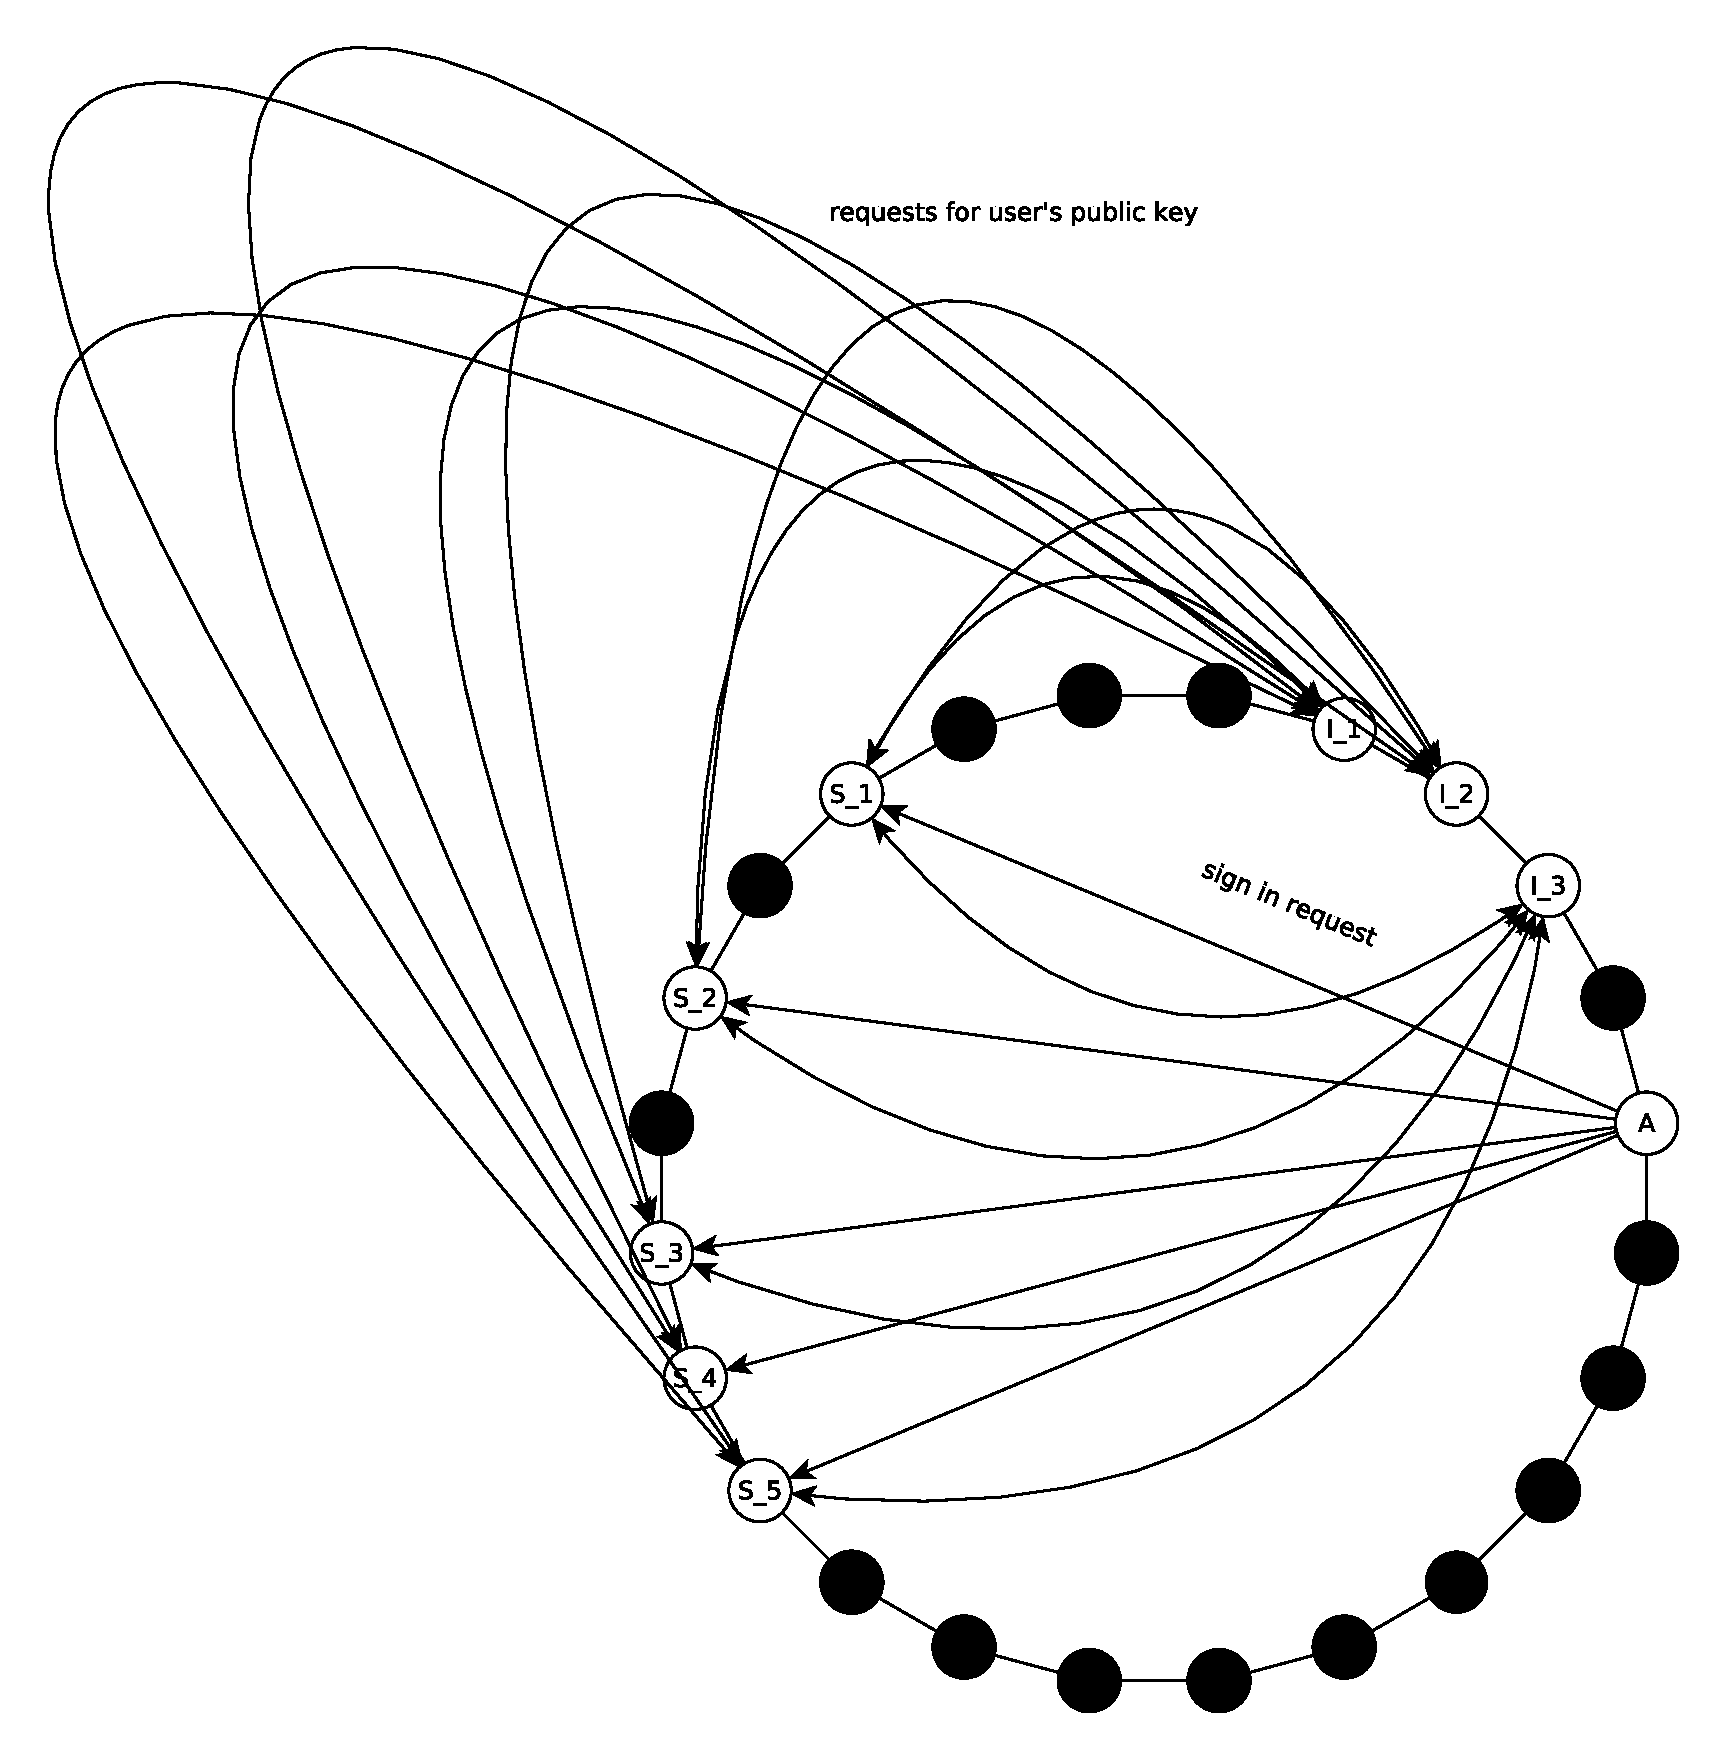
\includegraphics[height=0.7\textheight]{../../img/sign_in_2}
%\begin{table}
%\begin{tabular}{p{7cm}p{3cm}}
%&
%\vspace{1.5cm}
%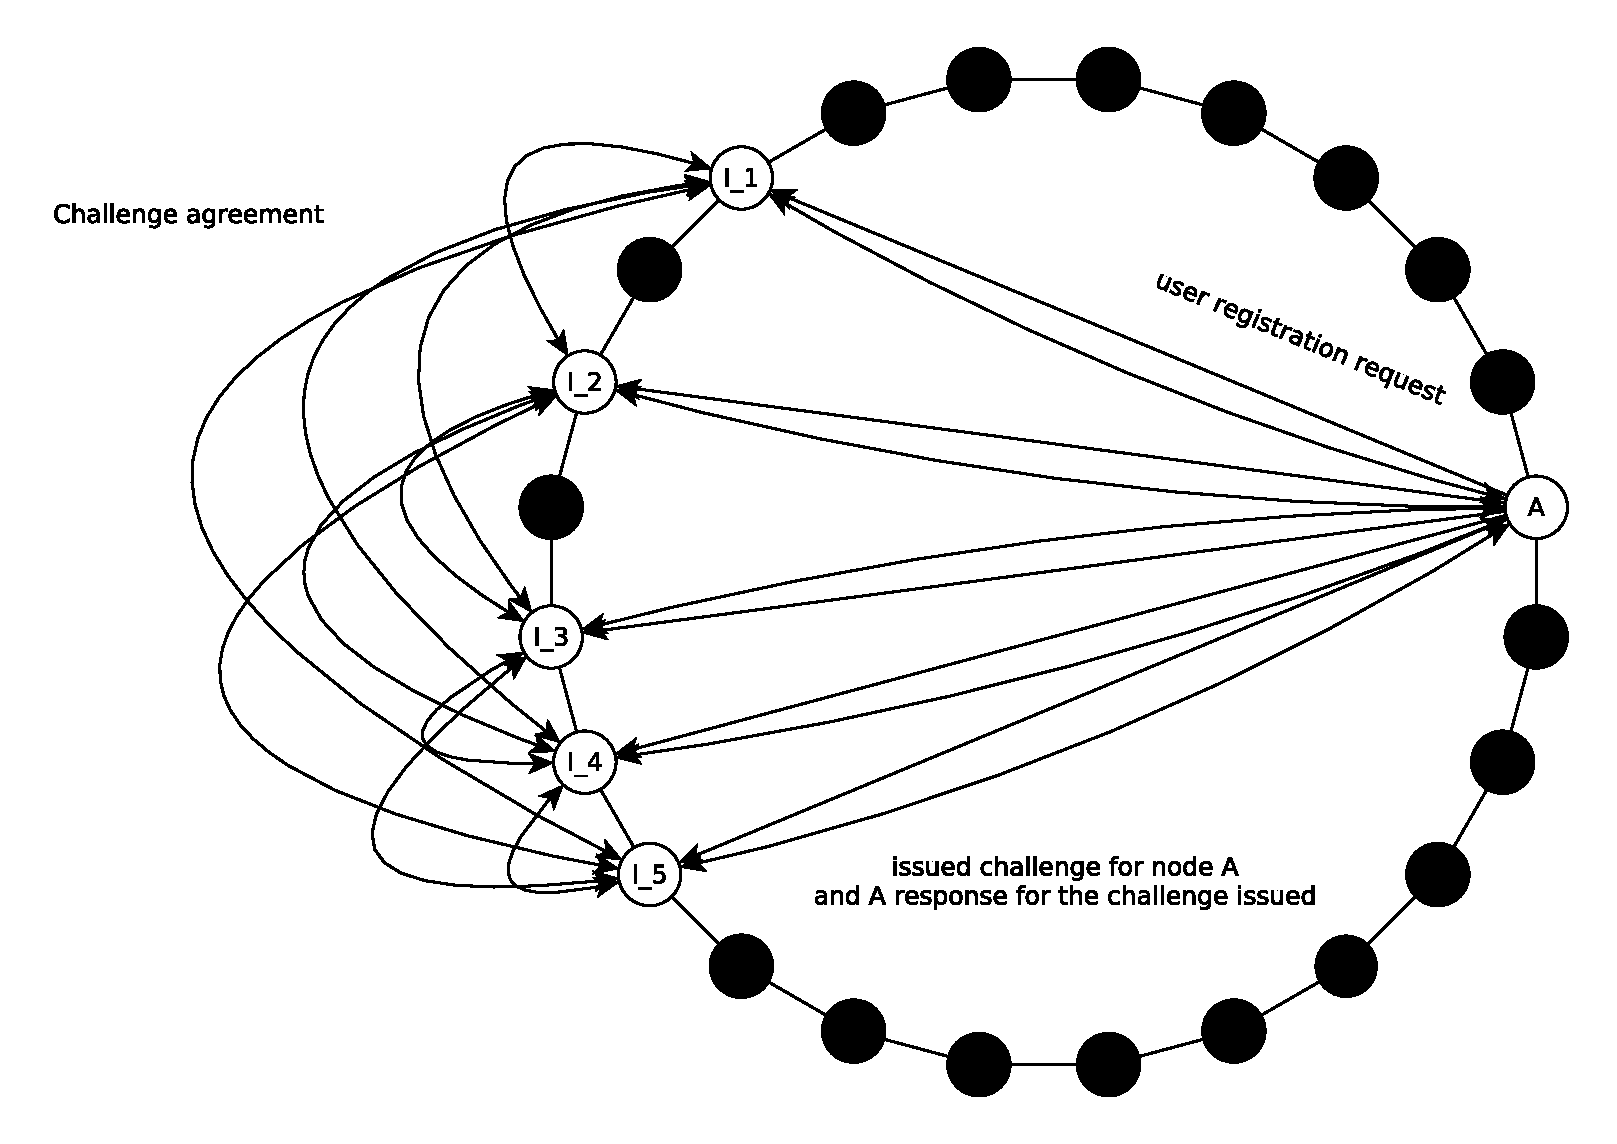
\includegraphics[width=4cm]{../../img/sign_up}\\
%\end{tabular}
%\end{table}
\end{frame}

\begin{frame}
\frametitle{System protocols}
\framesubtitle{User sign in (Generation of session keys)}
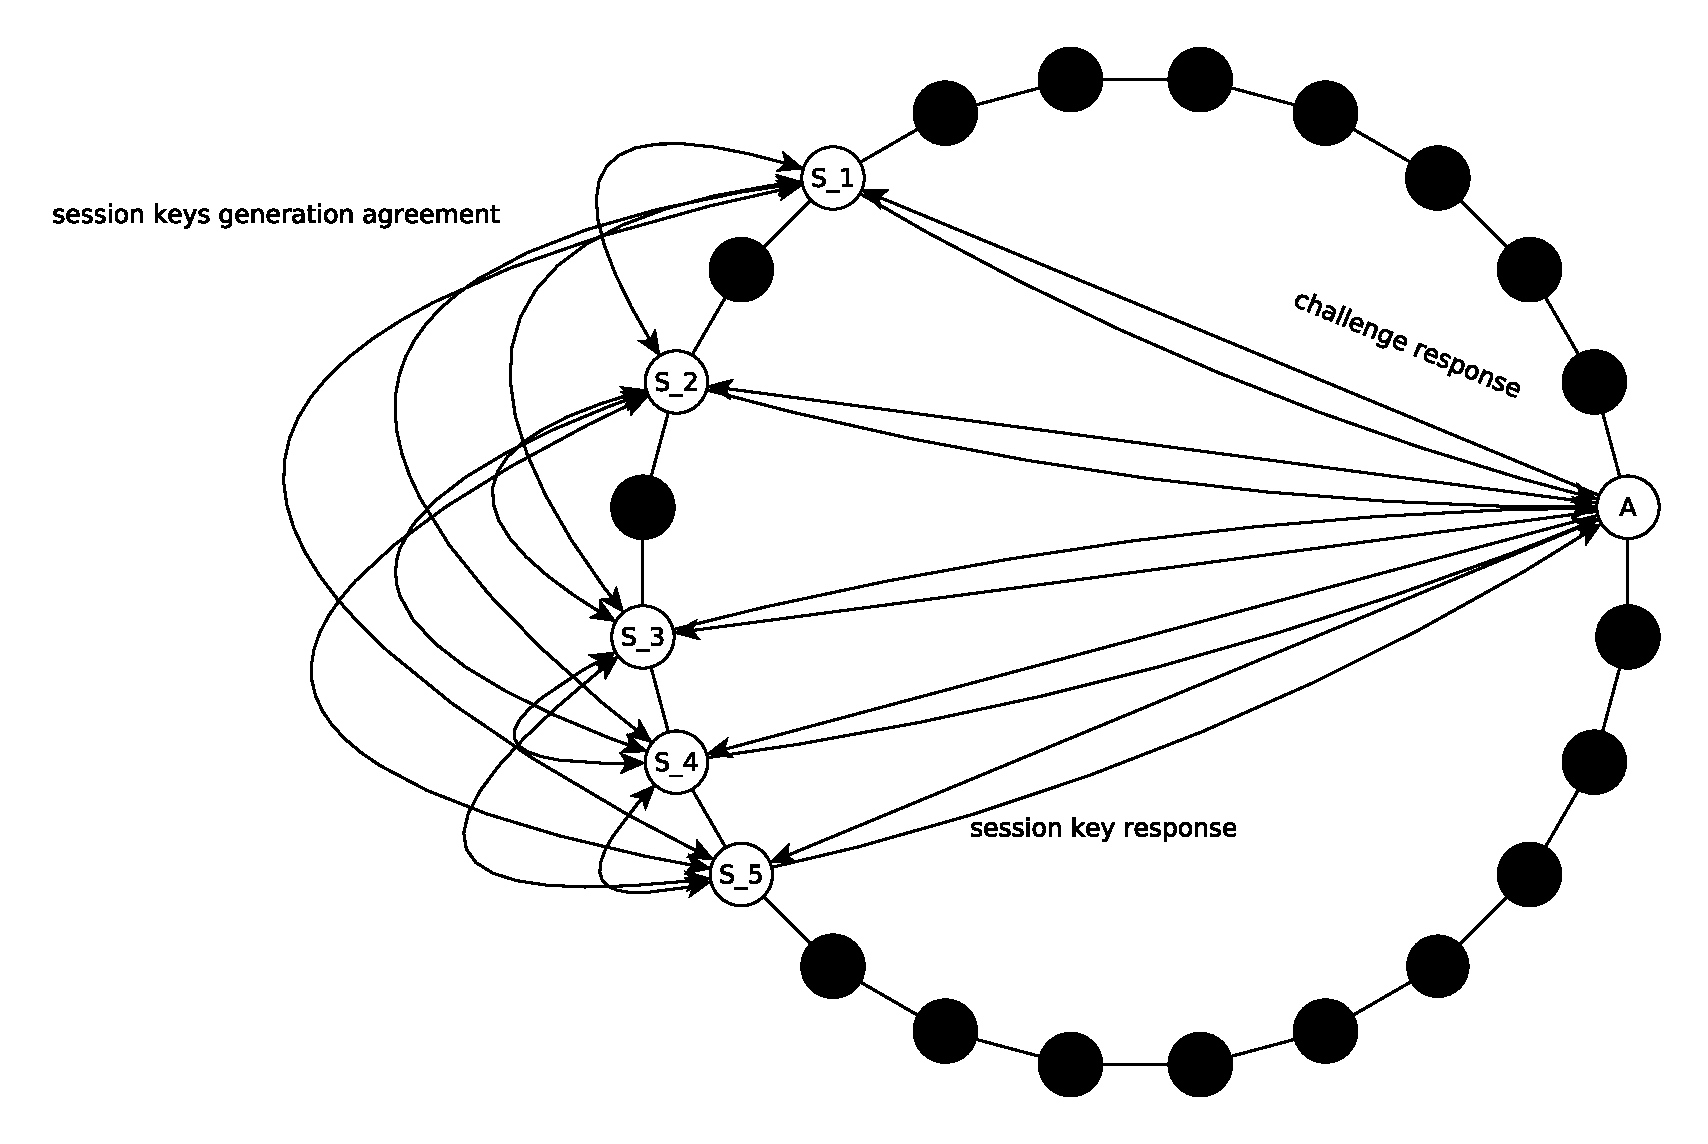
\includegraphics[height=0.7\textheight]{../../img/sign_in_3}\\
%\begin{table}
%\begin{tabular}{p{7cm}p{3cm}}
%&
%\vspace{1.5cm}
%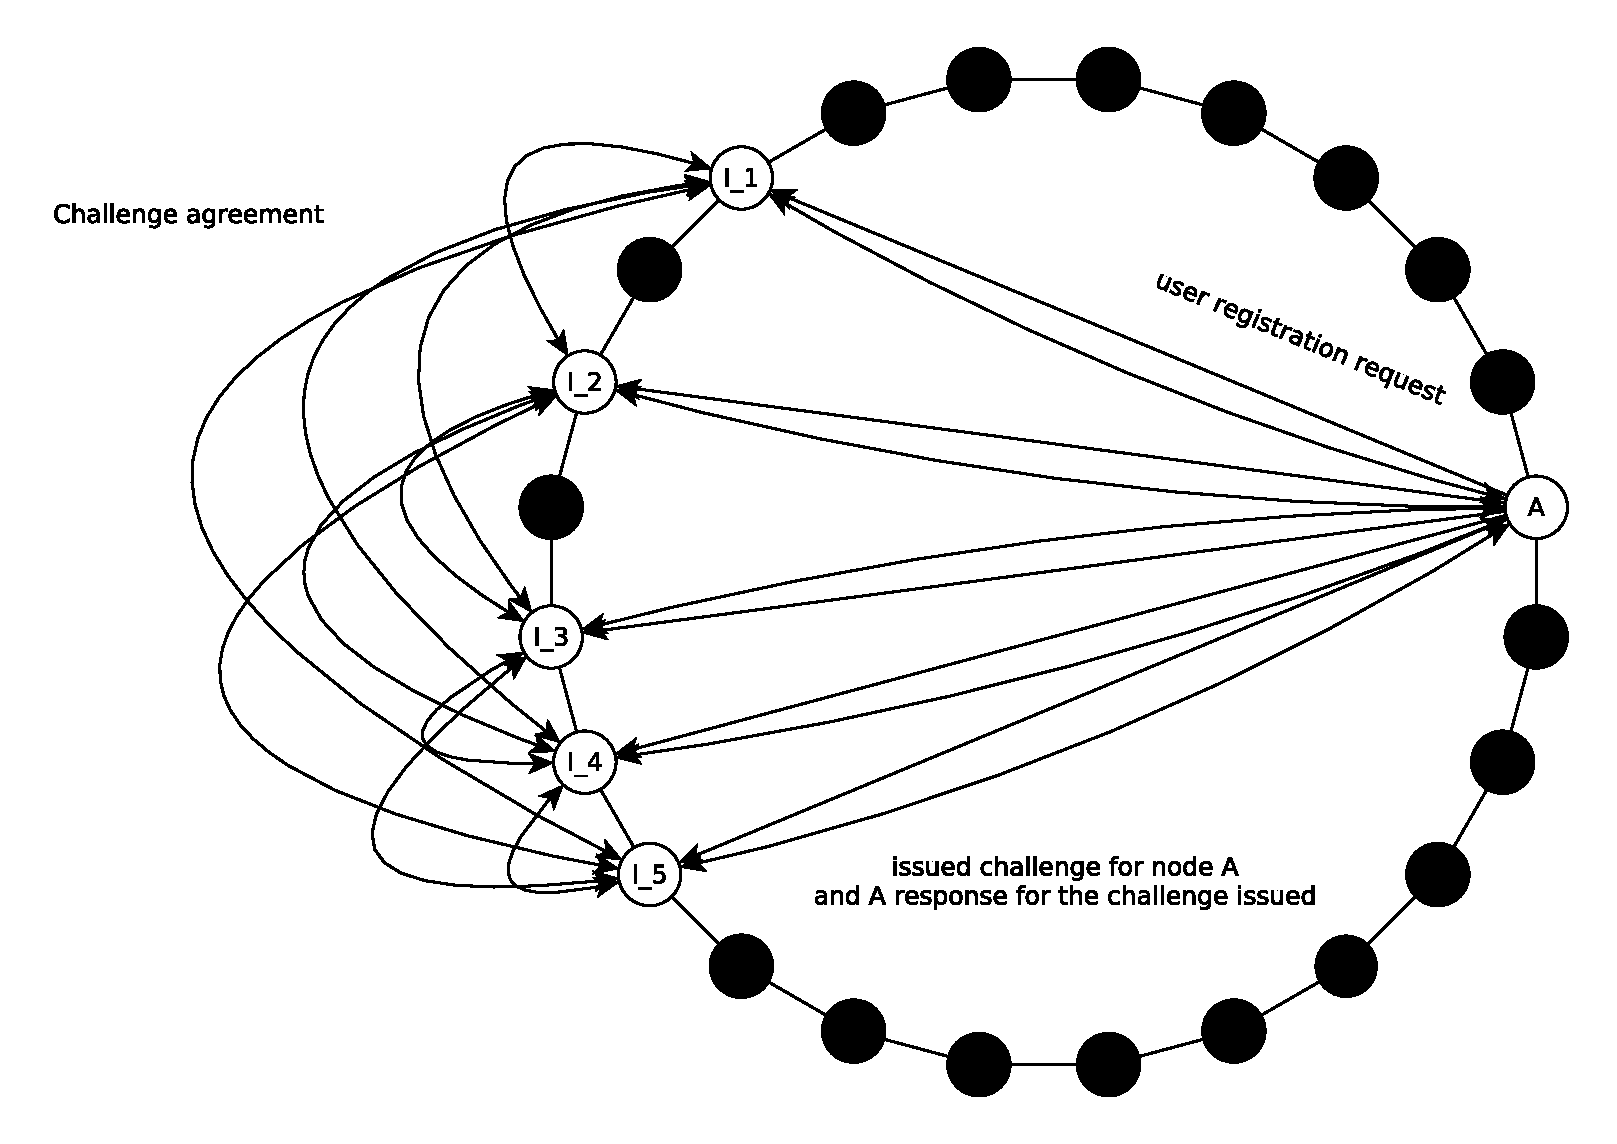
\includegraphics[width=4cm]{../../img/sign_up}\\
%\end{tabular}
%\end{table}
\end{frame}


\subsection{Logout, password change, user private key recovery}
\begin{frame}
\frametitle{System protocols}
\framesubtitle{More protocols}
\begin{table}
\begin{tabular}{p{7cm}p{3cm}}
\begin{itemize}
  \item Logout
  \item Password Change
  \item User private key recovery
\end{itemize}
&
\vspace{1.5cm}
%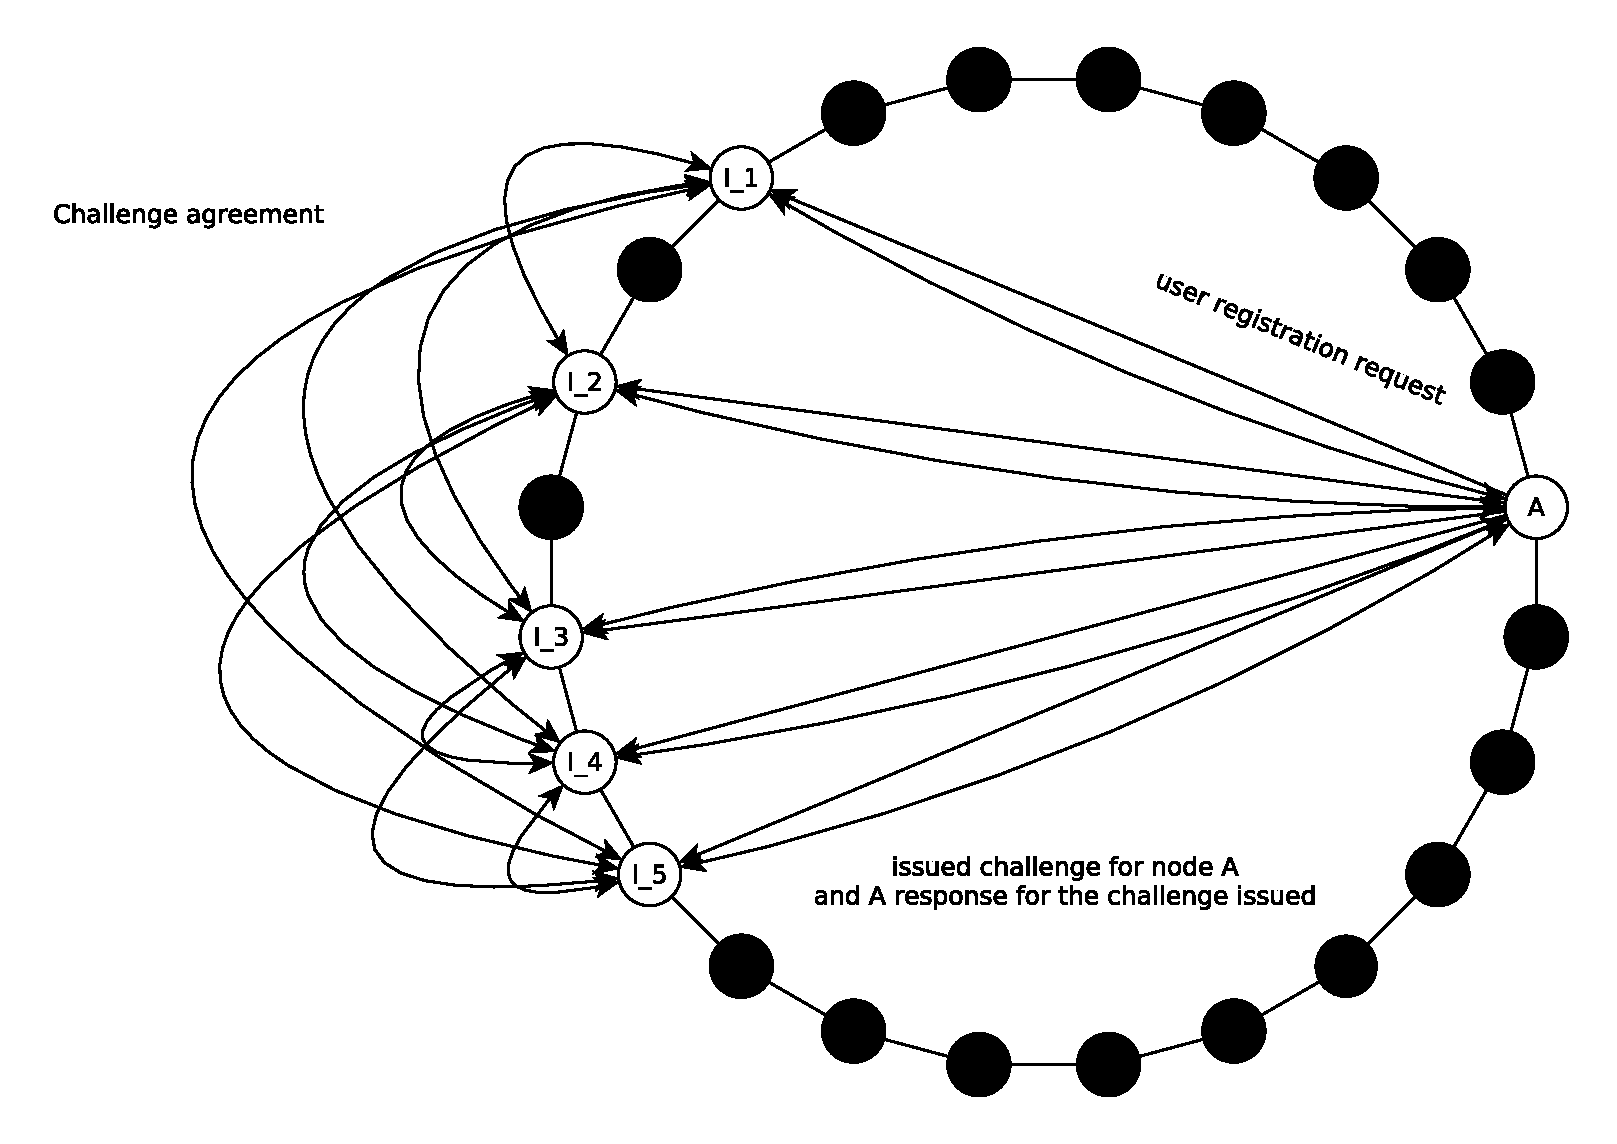
\includegraphics[width=4cm]{../../img/sign_up}\\
\end{tabular}
\end{table}
\end{frame}

\section{Evaluation}
\subsection{Parameters}
\begin{frame}
\frametitle{Evaluation}
\framesubtitle{Parameters}
  \begin{table}
    \centering
    \footnotesize
    \begin{tabular}{|ccc|}
      \hline
      \textbf{Parameter} & \textbf{Description} & \textbf{Value} \\
      \hline
      $\rho$ &  Probability of a node being malicious  & $0.3$  \\
      $\varepsilon$& CORPS classification error   & $0.05$ \\
      L &  Leafset/trustset size & $8$, $16$ or $32$  \\
      N &  Number of nodes in the DHT & $100000$  \\
      \hline
    \end{tabular}
    \caption{Parameters used for the evaluation of the protocols}
    \label{tab:variables_used}
  \end{table}
\end{frame}


\subsection{Probabilities of error}
\begin{frame}
\frametitle{Evaluation}
\framesubtitle{Probability of a system error/ protocol failure}
  \begin{table}
    \centering
    \footnotesize
    \begin{tabular}{|ccc|}
      \hline
      \textbf{Cases} & \textbf{System params} & \textbf{p value} \\
      \hline
      Worst case, no trusted nodes &  $L=8$  & $0.188$  \\
      Best case, no trusted nodes &  $L=32$  & $0.016$ \\
      Worst case, using trusted nodes &  $L=8$  & $6.64 \times 10^{-5}$ \\
      Worst case, using trusted nodes &  $L=32$  & $8.24 \times 10^{-14}$\\
      \hline
    \end{tabular}
    %\caption{Parameters used for the evaluation of the protocols}
    %\label{tab:variables_used}
  \end{table}
\end{frame}



\begin{frame}
\frametitle{Findings}
\framesubtitle{Theoretical results}
\begin{table}
\begin{tabular}{p{8cm}p{2cm}}
\begin{itemize}
  \item \textbf{Without trusted nodes:} With $p = 0.016$,\\
    \textbf{16000/1,000,000} failed transactions
  \item \textbf{Using a trusted set:} With $p =8.24 \times 10^{-14}$\\
    \textbf{0.00000000824/1,000,000} failed transactions
\end{itemize}
&
%\vspace{1.5cm}
%\includegraphics[width=4cm]{img/example}\\
\end{tabular}
\end{table}
\end{frame}

%
%\begin{frame}
%\frametitle{Findings}
%\framesubtitle{Theoretical results}
%\begin{table}
%\begin{tabular}{p{7cm}p{3cm}}
%\begin{itemize}
%  \item A system with $1000000$ users, with the probability
%of a protocol failure being $p = 0.016$,  $16000$ of the users will have problems with
%the protocols of the system. In comparison, with a probability of $p =8.24 \times
%10^{-14}$, of $1000000$ transactions only $0.00000000824$ would fail.
%\end{itemize}
%&
%\vspace{1.5cm}
%\includegraphics[width=4cm]{img/example}\\
%\end{tabular}
%\end{table}
%\end{frame}
%

\subsection{Conclusions}
\begin{frame}[allowframebreaks]
\frametitle{Conclusions}
\begin{itemize}
    \item while a 100\% secure implementation cannot be achieved, a viable solution exists.
    \item probability of error on the order of $10^{-14}$ can be achieved with a leafset size of $l = 32$.
    \item the system remains scalable.
    \framebreak
    \item the use of a reputation system and trusted nodes management mitigated the effectiveness of malicious node attacks in the network.
    \item a reputation system can also efficiently mitigate the effect of collusion attacks.
    \item computational challenges mitigate the problem of a node registering multiple users with the system.
      % reduce the probability from x to y? how this works?
%% comments
  % the system maintains a scalable cost when the size of nodes $n$ in the dht increases.
\end{itemize}
\end{frame}

  \section{Recommendations}
  \label{sec:recommendations}
  \begin{frame}
\frametitle{Recommendations}
\begin{table}
\begin{tabular}{p{7cm}p{3cm}}
\begin{itemize}
    \item 

%% COMMENTS
% Another issue that was not addressed is the bootstrapping of the P2P system.
% When the P2P system starts building up, there are no real trusted
% nodes and the services rely on just the few nodes that comprise the
% system. During that time there is a higher probability of failure of the protocols, and the system is
% more vulnerable to byzantine node attacks. Further research is still needed on
% that matter.

% Also, more research will be needed on new functionalities and addressing the
% problem of forgotten passwords and offline guessing attacks.

% While our system uses a username-password scheme for the user identification,
%we know that passwords presents serious security problems as the average user tends
%to use simple keywords and/or the same password in more than one service.
%A definitive solution to this problem has not
%been found yet. While a strict password creation policy can mitigate this
%problem, at the same time, it can also increase cases of forgotten passwords.
%Our proposed system does not implement password recovery mechanisms to reduce the 
%risks to the security of the system~\ref{sec:risks_password_recovery}.

%We also mention the use of
%additional challenges during user registration, like
%CAPTCHA to further increase resilience against Sybil attacks.\\

\end{itemize}
&
\vspace{1.5cm}
\includegraphics[width=4cm]{img/example}\\
\end{tabular}
\end{table}
\end{frame}

  %\section{Bibliografía}
  %\bibliography{src/url}
\frame
{
	\vspace{2cm}
	\begin{center}
		\Large{EOF}
	\end{center}
}
\end{document}
